\documentclass{sig-alternate}

\usepackage{listings}
\usepackage{hyperref}
\renewcommand{\topfraction}{0.9}
\renewcommand{\textfraction}{0.1}
\renewcommand{\floatpagefraction}{0.84}

\newenvironment{denseItemize}{%
\begin{list}{$\bullet$}{\setlength{\itemsep}{0in}\setlength{\parsep}{0in}\leftmargin=1em\labelwidth=1em}}{\end{list}}

\begin{document}
%
% --- Author Metadata here ---
\conferenceinfo{ICER 2013}{'13 San Diego, CA USA}
%\CopyrightYear{2007} % Allows default copyright year (20XX) to be over-ridden - IF NEED BE.
%\crdata{0-12345-67-8/90/01}  % Allows default copyright data (0-89791-88-6/97/05) to be over-ridden - IF NEED BE.
% --- End of Author Metadata ---

\title{An Open Platform for Managing Short Programming Exercises}

\numberofauthors{2}


\author{
\alignauthor
Andrei Papancea\\
Jaime Spacco\\
       \affaddr{Department of Computer Science}\\
       \affaddr{Knox College}\\
       \affaddr{Galesburg, IL 61401}\\
       \email{\{apapance,jspacco\}@knox.edu}
% 2nd. author
\alignauthor
David Hovemeyer\\
       \affaddr{Department of Physical Sciences}\\
       \affaddr{York College of Pennsylvania}\\
       \affaddr{York, PA 17403}\\
       \email{dhovemey@ycp.edu}
}

%\author{
%\alignauthor
%Author Name\\
%Author Name\\
%       \affaddr{Department of Computer Science}\\
%       \affaddr{Small College \#1}\\
%       \affaddr{City, State zipcode}\\
%       \email{\{author1,author2\}@school.edu}
%% 2nd. author
%\alignauthor
%Author Name\\
%       \affaddr{Computer Science Department}\\
%       \affaddr{Small College \#2}\\
%       \affaddr{City, State zipcode}\\
%       \email{author@school.edu}
%}


%\date{30 July 1999}

\maketitle
\begin{abstract}

We describe CloudCoder, an open platform for creating, assigning, and sharing
short programming exercises for a variety of languages (currently C/C++, Java,
Python and Ruby).  Like other similar systems, CloudCoder is web-based,
letting students write code directly in a web browser, click the
``submit'' button, and receive immediate feedback.  Unlike other
systems, which tend to be closed, or commercial, or both, CloudCoder
is a completely open platform.  The code for the system is
open-source, and exercises written for CloudCoder are shared to a
central repository under a permissive Creative Commons license
(BY-SA).  Finally, CloudCoder collects detailed data that faculty can use for
educational research.

In this paper, we report on successful pilot studies of CloudCoder at several
institutions.
% We also describe on-going work to create a ``hint'' system
%for CloudCoder, similar to what one would expect from an Intelligent
%Tutoring System (ITS).
We also outline some research questions we hope to address in future work.


% Students access CloudCoder exercises 
% through their web browser, where they can edit code

% Importance of understanding code more deeply.

% Identify ``knowledge components''

% Identify when and where to insert hints

% (Maybe) use Euclidean distance to compute closeness of two solutions

% To generate hints:  What hints to generate, when to generate them

\end{abstract}

% A category with the (minimum) three required fields
\category{K.3.2}{Computers and Education}{Computer and Information
  Sciences Education}[Computer Science Education]

\terms{Human Factors, Measurement}

\keywords{CS1, novice programmers, data collection, student behavior}

\section{Introduction}

Recent years have seen an explosion of online services for learning
to program:  Udacity \cite{udacity}, Codecademy \cite{codeacademy},
ProgZoo \cite{progzoo}, 
Codingbat \cite{codingbat}, Coursera \cite{coursera}, Turingscraft
\cite{turingscraft}, Problets \cite{Kumar:2005:GPA:1163405.1163408}, CS Circles \cite{Pritchard:2013:CCI:2445196.2445370} and
several others.  These systems are very powerful, and show great promise to
improve introductory computer science.  Given all of these
very good systems, one may ask why we thought
%it a good career move
%to build yet another system.
the world needed another such system.

%There are three main reasons:
%
%%\begin{itemize}
%
%%\item 
%First, we wanted a system that an instructor can easily integrate into an existing traditional course.
%  Many massive open online courses (MOOCs), such those available through Udacity and
%  Coursera, were not designed for a traditional classroom and cannot be easily incorporated into an existing course.  
%  The infrastructure provided by a MOOC is geared towards the course
%  taught through the MOOC, and is not really configurable or customizable.
%
% % systems, such as Udacity, Coursera, and CodeAcademy, are
% %  massive open online courses (MOOCs) that cannot be easily
% %  incorporated into a traditional classroom setting.  MOOCs can be wonderfully
% %  enriching for students who take these courses.  However, because
% %  MOOCs offer an entire
% %  course, whatever online programming infrastructure they provide is part of that
% %  course.
%
%%\item 
%Second, we wanted an open, customizable system that focuses on short programming exercises that students
%  can solve in their browser, and receive immediate feedback.  There are excellent systems that help
%  faculty manage longer programming assignments
%  \cite{Edwards:2008:WAG:1384271.1384371}, or homework and review questions
%  \cite{turingscraft, Kumar:2005:GPA:1163405.1163408}.  Codingbat
%  \cite{codingbat} is a fantastic free service that provides short
%  programming exercises, but it is not easily customizable and does not provide
%  access to all of the submissions submitted by students.
%  We see CloudCoder as a complementary component to these resources.
%
%% Some existing systems, such as Problets \cite{Kumar:2005:GPA:1163405.1163408},  and Turingscraft
%%   \cite{turingscraft}, provide homework exercises that can be incorporated
%%   such as Codingbat \cite{codingbat},
%%  , can be integrated into an existing course.
%%   Codingbat, while free to use and fantastically useful, does not give faculty access to a very
%%   rich data set
%
%%\item
%Finally, we wanted exercises that could be freely modified and
%redistributed.  Much of the excellent content available through MOOCs,
%or the increasing amount of digital content available through textbook publishers, 
%cannot be modified or re-used outside of those contexts.  This can be a significant
%impediment to researchers trying to study the difficulty level of
%various exercises, or to build intelligent tutoring systems (ITSs)
%that require a large bank of questions and their solutions.
%
%%\end{itemize}
%
%% There are two reasons.  First, many of
%% these systems, such are Udacity, Coursera, and CodeAcademy, are
%% massive open online courses (MOOCs).  MOOCs typically provide
%% supporting infrastructure that helps students learn to code in their
%% browsers, and the course material offered by a MOOC can be a wonderfully enriching
%% experience for someone who enrolls in the course.  However, it is not
%% clear how faculty who teach more traditional courses can
%% integrate any of the infrastructure provided by a MOOC into
%% their curriculum.  Second, 
%% the systems that could be easily integrated into an existing course, such as
%% Codingbat or Turingscraft, are
%% are either commercial, or closed, or both.  To our knowledge, none of
%% these systems readily support faculty who want to 
%% modify the code, host their own installation, extract data about
%% student behaviors beyond the basic correctness of their submissions,
%% or redistribute the programming exercises and assignments.
%
%We believe the academic community should have a fully open alternative
%to the closed and/or commercial systems that have exploded onto the CS
%Education scene.  Faculty can integrate CloudCoder into an existing course with minimal overhead,
%can write their own content, use and modify content contributed by
%others, customize the system, and collect data for educational studies.

Our primary motivation was {\em freedom}: we wanted a system where
the software and exercises could be freely redistributed, and
were not under the control of any central authority.  This motivation
is not entirely philosophical: we felt that locking down either
the software or the exercises would result in a barrier to adoption,
limiting the potential impact of the system.
As we will discuss in Section~\ref{sec:questions}, we think that there
are some interesting research questions that can be addressed
best through the existence of a ``free like air'' programming
exercise system: for example, we are very interested in finding out
whether exercises can be reused effectively in different courses
at different institutions.

Another motivation was a desire to collect data on students' work
on programming exercises as a way to study how students learn to program.
For example, CloudCoder captures a fine-grained edit history of each
student's work on each exercise.  Because the system is open source,
we (and other researchers) can easily add other kinds of data collection
to the system.

Finally, we wanted a system that supported a wide range of programming
languages.  For example, relatively few programming exercise systems
support C and C++.


\section{CloudCoder}
We have designed CloudCoder to be an open platform for managing short
programming exercises.  The CloudCoder platform has four design
goals:  To be an open-platform for faculty to assign short programming
exercises, to build a collection of redistributable programming
exercises, to collect data about student behaviors as they solve
exercises, and to explore ways of curating the collected data.

% \begin{itemize}
% \item {\em To provide a web-based platform for faculty to assign short
%   programming exercises.}  

% There are platforms such as Web-CAT \cite{Edwards:2008:WAG:1384271.1384371},
% 
%  TODO Insert Marmoset reference!
%
 % and the many in-house systems developed at universities, for managing longer programming
 %  assignments, and there are commercial systems such as Turingscraft
 %  for assigning online homework \cite{turingscraft}.  However, there
  % are currently no open, flexible systems that serve a similar
  % purpose.  All of the code is open-source and available at Github:


% \item {\em To crowd-source the construction of a repository of programming
%   exercises.}  
% \item {\em To collect data about student work on short
%   programming exercises.}  There are many systems that collect data
%   about novice programmers \cite{Utting:2012:WDG:2361276.2361278,
%     Jadud:2006:MTE:1151588.1151600, Norris:2008:CCQ:1384271.1384284,
%     Spacco:2006:EMD:1140124.1140131}. % TODO: Cite French paper on Eclipse plugin
%   However, these systems typically target longer programming
%   assignments that students spend a week or two working on.
%   CloudCoder target very short exercises, and logs data at the
%   keystroke level.  We envision faculty using CloudCoder as a platform
%   for educational studies that require studying fine-grained trace data.
% \end{itemize}

\begin{figure*}
\centering
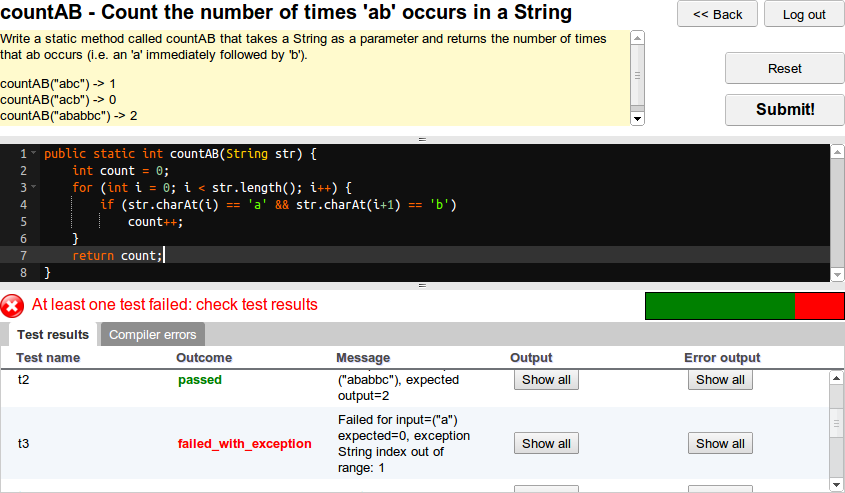
\includegraphics[width=5.5in]{images/screenshot4}
\caption{Screenshot of the main view in CloudCoder}
\label{screenshot}
\end{figure*}


\subsection{An Open Platform}

CloudCoder is an open platform for managing short programming
exercises.  Each exercise can be solved with one method or one short
program, and could take only a few minutes to solve, or could require
or an hour or two.  The system is not designed to support longer
programming assignments, such as those found at the {\em Nifty
Assignments} session at SIGCSE.

Figure~\ref{screenshot} shows a screenshot of a CloudCoder exercise.
The editor is derived from the Ace editor \cite{ace}, and supports
syntax high-lighting for most programming languages, and
auto-indentation.  
A submit button runs the code against a series of
test cases, and feedback is provided directly in the browser.
CloudCoder captures anything the code prints to standard out or
standard err to help students with debugging.

\begin{table*}
\centering
\begin{tabular}{| l | l | l | l |}
\hline
Institution & Course & Language & Enrollment\\
\hline
Canisius College & CS-1 & C/C++ & 30\\
York College & CS-1 & C/C++ & 120\\
Knox College \#1 & CS-1 & Java & 23\\
University of Auckland & Programming for Engineers & C & 30\\
\hline
\end{tabular}
\caption{CloudCoder pilot studies.}
\label{tab:courses}
\end{table*}

CloudCoder is available under the GNU Affero open-source license.
Binary distributions are available through our website (\url{http://cloudcoder.org}),
and the code is available on Github:

\vspace*{3mm} 
\url{https://github.com/cloudcoderdotorg/CloudCoder}
\vspace*{3mm}

% The editor window 

\subsection{Permissively-Licensed Exercises}

Writing good homework exercises is difficult and
time-consuming, and even the best textbooks are limited in the
number and quality of practice exercises they can provide, to say
nothing of a textbook's inability to provide timely feedback to
students.
Sharing exercises between faculty members is a much
more efficient way to increase the number and quality of exercises at
our disposal.

Faculty who use CloudCoder can write their own exercises using our in-browser
authoring tools, or can import exercises written by other faculty
from a central repository at:

\vspace*{3mm} 
\url{https://cloudcoder.org/repo}
\vspace*{3mm} 

Currently we have over 50 Java and 60 C/C++ exercises authored by 5
different users.  By default,
any new exercises written by faculty will be shared to the 
central repository under a permissive Creative Commons license (BY-SA)
that allows redistribution provided that the author is credited and
redistribution is under the same license.  
(Note that the repository shows the exercise description, but not the
test cases or the solution, so an unscrupulous student cannot dig through the
repository for solutions.  Importing exercises requires an account at
the repository, which can be used to discourage this sort of
undesirable behavior.).

CloudCoder supports two types of exercises:  {\em method} or {\em function-based}
exercises, and {\em whole-program} exercises.  Function based exercises look
a lot like Codingbat exercises:  Students are given a description of
what the method should do, and a couple of example input/output pairs
similar to a unit test.  Writing a new function-based exercise
requires a description, some ``starter code'' (typically the method
header, although exercises can provide as much or as little code as
desired), and a series of inputs and their corresponding outputs.
Test-cases can be marked as ``secret'' so that students don't see their
outputs to discourage students from writing a special case to
recognize each input.

On the other hand, whole-program exercises
have a description, but read inputs from
standard-in and write to standard-out.  CloudCoder uses a
simplified regular expression language to check student outputs for
correctness.


\subsection{Building and Testing Submissions}

CloudCoder currently supports exercises for C/C++, Java, Python and
Ruby.  Building and testing takes place in a separate process which
can be run on a separate machine for extra security, or on multiple
machines for scalability.

We run Java code relatively securely under a Security Manager, and 
use Jython and JRuby to compile Python and Ruby to Java
bytecode, which we also run in a Security-Managed sandbox.  We
currently support C/C++ less securely, although 
recent work by Malan \cite{Malan:2013:CSS:2445196.2445242} on a
``sandbox'' for running untrusted student code can be leveraged to improve our security.


\subsection{Data Collection and Curation}

CloudCoder logs keystrokes in the online editor window, and 
stores all submissions and test outcomes in a databases.
We hope that the combination of exercises and data will give faculty
insights into the difficulty level of different exercises, keep a
record of common error patterns, and enable the development of
innovative data analyses.


One question is how to manage the data collected.  
Recent work on web-scale data collection by the BlueJ team
\cite{Utting:2012:WDG:2361276.2361278} lays out a number of important
questions about programming data, such as who should have access to the data, and what
mechanism should be used to access the data.  Sanders
et. al. \cite{Sanders:2008:DSE:1404520.1404534} reviewed a number of
the challenges involved in sharing empirical education data.  

An alternative repository for the type of data collected by CloudCoder
is the Pittsburgh Science and Learning Center (PSLC) Datashop, which
is a repository of data collected by by intelligent tutoring
systems (ITSs).  By its nature, ITS data is much simpler than program
snapshot data, so snapshots cannot be added without some changes.
The Datashop is interested in storing program
snapshot data to make it easier for researchers in the ITS, educational data
mining, and CS-ed communities to work on programming data.

Anonymized data that has been cleared by the proper Institutional
Review Boards is contributed to the Datashop, which
makes the data available to other researchers under whatever
restrictions were put in place by the overseeing IRBs.  The Datashop also
provides a suite of analysis and visualization tools for better making
sense of the ITS data.

We are working with members of the Datashop to establish standards for
program snapshot datasets, and to begin developing tools and
techniques that can help analyze this very different dataset.  This is
a long-term project that is in its infancy.

% The Datashop stores traces from ITSs, which are typically made up of
% multiple choice questions, and merely need to store a student's
% answer, and whether they asked for a hint.  

% We have been in contact with the the Pittsburgh Science and Learning
% Center (PSLC) Datashop.  The Datashop is a repository for 

% The data collected by CloudCoder is simpler than the data collected by
% the BlueJ team.  

%Standard storage formats, visualization tools, standard analyses.

\subsection{Hosting CloudCoder}
We recognize that ease of installation is a critical factor for
adoption of a new pedagogical
technology for busy
faculty who may only have a few minutes to evaluate a new system.  We
are committed to making the installation process as simple and painless as 
possible.

Thus far each institution that has adopted CloudCoder has
provided a Linux server that we configured for them.  This has made
adoption very easy, but is unlikely to scale up as we acquire more
users.  We have asked Amazon for Amazon Web Services credits to
provide CloudCoder ``in the cloud'' to adopting institutions, and we
hope to add support for Google App Engine this summer.  Ease of
adoption is critical for CloudCoder.

\subsection{Pilot Studies}

We piloted CloudCoder at several institutions during the 2012-2013
academic year.  Table~\ref{tab:courses} shows a breakdown of the
courses.  We tried to use CloudCoder at Auckland in Fall 2012 for a
course with 700 students, but the free-tier of Amazon EC2 did not
scale up well enough, so we only recorded partial data.  We have made
significant improvements since then and plan to deploy CloudCoder for
the same large course in Fall 2013.


In the Winter 2013 term at Knox College, students taking CS-1 used {\tt CloudCoder}
%
% TODO: \cite{Hovemeyer:2013:CBC:2445196.2445451}.  
% 
We collected over 6,000 submissions
for 32 exercises by 23 students.  We expect to have a much larger
dataset from 120 students at 
York College 
once the Spring 2013 semester ends.  Our analysis of these datasets is
very preliminary at this point, but work is ongoing.


\section{Questions}\label{sec:questions}

%We could use community input into the CloudCoder project.  Specifically:
%
%\begin{itemize}
%\item Who would be interested in adopting this system?  If you would
%  consider trying out the system if we added a particular feature,
%  what would that feature be?  We would like
%  to expand our pilot group.
%\item What studies could or should be done with this platform?  And
%  would you like to be involved with these studies?
%\item What studies can be done with the existing data we have
%  collected?  We do not yet have well-developed tools for data
%  analysis, but one data set has been anonymized and can be
%  distributed to other researchers interested in our data.
%\end{itemize}

There are a number of questions, both research-oriented and philosophical,
that we would like to address in the context of our future work with CloudCoder.

{\bf Can the adoption of programming exercises lead to improved outcomes
in introductory programming courses?}  This is the most obvious
question.  One scenario we are particularly interested in is whether
the use of programming exercises, when {\em added} to an existing course with
no other changes in pedagogy, can result in improved outcomes.  We feel
that this scenario is important because educators have limited time
and resources available to change the way their courses are taught.
If programming exercises are an easy change to implement, then
if adopted on a wide scale they could have a significant impact.

{\bf Can exercises be reused effectively outside of the course in which
they were originally created?}  When assigning a programming exercise to
students, the instructor can create one from scratch, or use a
previously-written exercise.  Since creating good exercises is labor-intensive,
being able to use a previously-written exercise represents a significant
time savings.  However, finding an existing exercise that is {\em appropriate}
is not necessarily a trivial task.  We are interested in finding
out whether exercises written in the context of one course can be reused
effectively in another.
This question has several interesting aspects:

\begin{denseItemize}
\item How can we help instructors search for appropriate exercises?
\item How can we classify exercises?
\item Can we allow CloudCoder users to {\em improve} existing exercises?
\end{denseItemize}

{\bf What guidance can we provide to instructors on which exercises to assign,
and in what order?}  This question is an expanded form of the previous question:
if a large repository of pre-written exercises is available,
could we offer instructors sequences of exercises on a particular topic?

{\bf How can programming exercises be integrated most effectively into a course?}
Programming exercises can be used for many purposes: self-test questions
to accompany readings and video lectures, in-class assessment (possibly
in the context of peer instruction), extra practice for students who
are struggling.  We would like to have specific, evidence-based recommendations
that we can give to instructors who are considering using programming
exercises in their courses.

{\bf Given an effective mechanism for sharing curriculum materials, could
courses at a number of institutions converge towards an optimum?}
This question is more philosophical, and is based on the observation that
curricula and pedagogy vary widely between instructors and institutions,
even for the ``same'' course \cite{Hertz:2010:CCM:1734263.1734335}.  We find ourselves wondering
if more effective ways ways of sharing curriculum materials would lead
to the best materials and ideas propagating widely, and if high-quality introductory
programming courses could created as a ``mash-up'' of materials created by
many authors at many institutions.  CloudCoder and similar systems
could be one mechanism enabling this type of transfer.

{\bf Should exercises be graded?
If exercises are shared freely, is the availability of solutions a concern?}
These questions are related: if exercises are available publicly,
solutions will likely be available publicly as well.  (For example,
many if not all CodingBat problems have solutions which can be found
through a web search.)  If exercises are graded, then some students may
choose to cheat rather than attempt to solve the problem honestly.

{\bf What are appropriate incentives to encourage students to attempt
the exercises (and get the maximum benefit from them)?}
If exercises are not graded, then what incentives can be used to
encourage students to make a serious attempt at solving them?

{\bf What is the right balance between short programming exercises and
  longer ``nifty'' assignments?}
Discuss.

{\bf What can we do to encourage students to use their time effectively outside of class?}

\section{Related Work}

Jadud's pioneering early work on novice compilation behavior
\cite{Jadud:2006:MTE:1151588.1151600}, along with follow-up work by
others \cite{Norris:2008:CCQ:1384271.1384284} provides a starting point for
work with program snapshots.

Denny et. al. have studied novice syntax errors
\cite{Denny:2012:SEE:2325296.2325318} using data collected from the CodeWrite system.
CodeWrite is similar to CloudCoder, except that students create
exercises and test cases for each other to solve, and are evaluated on
the quality of their practice exercises.

Lane et. al. describe Intention-Based Scoring (IBS) \cite{Lane:2005:ISA:1047344.1047471},
an approach to building an ITS for programming whereby human
judges to score or code {\em charettes}, or assignments students work on in a
timed, closed-lab environment.  IBS derives from prior work on
identifying ``bugs'' in online protocols, and as such attempts to
identify places where students have a ``bug'' in their development
process.  This approach, while labor-intensive, shows some promise in
developing an ITS for programming assignments.

Zingaro et. al. built the Python Classroom Response System
\cite{Zingaro:2013:FCP:2445196.2445369}, a system similar to
CloudCoder, except that it focuses on supporting in-class programming
questions for a class that uses a {\em Peer Instruction} pedagogical approach.

Pritchard et. al. present CS Circles
\cite{Pritchard:2013:CCI:2445196.2445370}, an interactive on-line
Python curriculum that embeds short questions, some of which involve
programming, directly into the text.  This sort of interactive text
shows great promise for developing open, interactive courses.

The BlueJ team presents a compelling case for web-scale data
collection \cite{Utting:2012:WDG:2361276.2361278}.  Their system is
more ambitious than CloudCoder, but the data collected by CloudCoder
should be complementary.

%
%\section{Future Work: Towards an Intelligent Tutoring System}
%
%One of the long-term goals for CloudCoder is to use the data to
%develop an Intelligent Tutoring System for programming assignments.
%A web-based programming ITS could be used to support high school
%AP courses in school districts that may lack computer science
%teachers, or to help improve introductory CS courses by reducing
%student frustration.
%
%To develop an ITS, we need a large supply of exercises; we hope
%CloudCoder's permissible licensing will help on this front.  We also
%need to provide students with ``hints'' when they are stuck.  To
%provide hints, we can either write the hints ourselves, which is
%labor-intensive, or generate them automatically by mining them out of
%the dataset of prior submissions.  Obviously this second approach is
%a much preferred method of creating hints.  However, identifying hints
%automatically means that we need to match a student's current program
%state with the most similar program state we've seen previously, 
%figure out what successful next step the previous student took, and
%then summarize this information into a hint.  This is a very
%challenging problem.
%
%There are currently two promising lines of research
%trying to address the issue of identifying the most similar previous submissions.  Rivers and Koedinger \cite{rivers-its2012} have developed a
%system that computes a {\em canonicalized} version of each submission
%by compiling to an Abstract Syntax Tree (AST) and then applying a
%series of compiler transformations.  This work is ongoing, but
%preliminary results are encouraging.
%On the other hand, Jin et. al. \cite{Jin:2012:PRA:2345840.2345889, jin-kdd2011} perform
%an inter-procedural data flow analysis that tracks the values stored
%in different variables in an effort to identify variables that are
%used in the same way in each submission.  They also show promising preliminary
%results for their approach.
%
%\subsection{Key Features:  Mining Hints from the AST}
%
%Our approach, which is very preliminary, ongoing research,  is also based on an analysis of
%the AST.
%Our hypothesis is that many novice-level exercises
%will have solutions that require certain structural
%{\em key features} in the code that we can detect automatically by
%comparing the AST of the student's code with the ASTs of known correct
%solutions.
%
%For example, Figures~\ref{fig:counta} and \ref{fig:countab} show two
%CloudCoder exercises that were assigned during the Winter 2013 term in
%CS-1 at 
%Small College \#1
%%Knox College.
%
%\begin{figure}[h]
%{\tt Write a static method called countA that takes a String as a
%parameter and returns the number of times that 'a' occurs in the String. }
%\caption{CountA:  An example CloudCoder exercise.}
%\label{fig:counta}
%\end{figure}
%
%
%\begin{figure}[h]
%{\tt Write a static method called countAB that takes a String as a
%parameter and returns the number of times that ab occurs (i.e. an 'a'
%immediately followed by 'b'). }
%\caption{CountAB: Another example CloudCoder exercise.}
%\label{fig:countab}
%\end{figure}
%
%First let us consider the {\tt CountA} exercise from
%Figure~\ref{fig:counta}.  As is typical in computer science, students have a lot of flexibility
%in how they solve this problem:  with a for loop or with a while loop, using the {\tt charAt()}
%method or the {\tt substring()} method or other String methods, and so on.  However, in
%practice, exercises are assigned in a context with other
%exercises, in-class examples, and course topics, which tends to limit
%the scope of possible student solutions, and to push students towards
%certain solutions and away from others.  For example, no student solved this
%exercise with a while loop, and all but one used {\tt charAt()}
%rather than other String operations.  In fact, most correct
%solutions looked something like Figure~\ref{fig:counta-solution}.
%
%\begin{figure}[h]
%\begin{lstlisting}
%public static int countAB(String str) {
%  int count=0;
%  for (int i=0; i<str.length();i++) {
%    if (str.charAt(i)=='a') {
%      count++;
%    }
%  }
%  return count;
%}
%\end{lstlisting}
%\caption{Typical solution for Exercise CountA depicted in Figure~\ref{fig:counta}.}
%\label{fig:counta-solution}
%\end{figure}
%
%
%\begin{figure}
%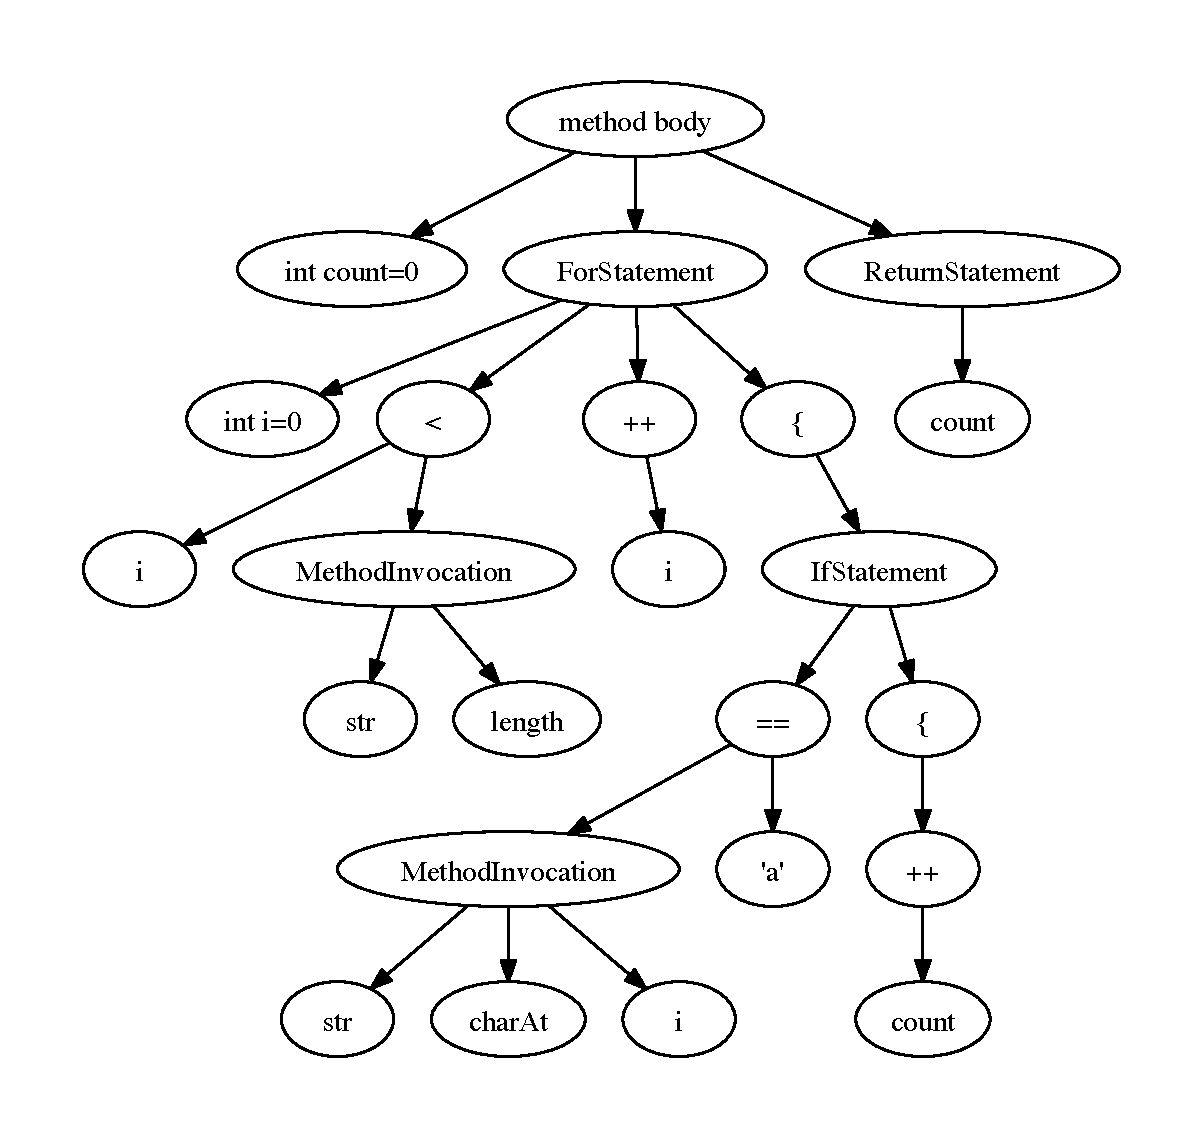
\includegraphics[width=90mm]{images/countA.pdf}
%\caption{Slightly simplified AST of the code in Figure~\ref{fig:counta-solution}}
%\label{fig:counta-ast}
%\end{figure}
%
%Compiling the method from Figure~\ref{fig:counta-solution} to an
%Abstract Syntax Tree (AST) produces a tree that looks something like
%Figure~\ref{fig:counta-ast} (the AST has been simplified slightly by
%collapsing nodes that are unimportant for this example).  We can identify
%several features of the AST that must be present to solve the
%exercise, such as a for loop, an if-statement inside the loop, and
%the use of a String method, typically {\tt charAt()}, to examine
%characters inside the loop.  We can also ensure that the components of
%the for loop are correct, i.e. that the loop counter starts at 0, that
%the loop goes up to the length of the String, and so on.  Assuming
%that student code compiles, all of these necessary features can be
%extracted from the AST. 
%
%Now let's consider the {\tt CountAB} exercise depicted in
%Figure~\ref{fig:countab}.  Again, there were many correct solutions;
%however, many correct solutions looked something like
%Figure~\ref{fig:countab-solution}.  
%
%\begin{figure}[h]
%\begin{lstlisting}
%public static int countAB(String str) {
%  int count=0;
%  for (int i=0; i<str.length()-1;i++) {
%    if (str.charAt(i)=='a' && 
%        str.charAt(i+1)=='b') {
%      count++;
%    }
%  }
%  return count;
%}
%\end{lstlisting}
%\caption{Typical solution for Exercise countAB depicted in Figure~\ref{fig:countab}.}
%\label{fig:countab-solution}
%\end{figure}
%
%Compiling the method in Figure~\ref{fig:countab-solution} into an
%abstract syntax tree (AST) produces a tree that looks like
%Figure~\ref{fig:countab-ast} (this result has been slightly simplified
%from the full output from the Eclipse JDT compiler).
%
%\begin{figure}[h]
%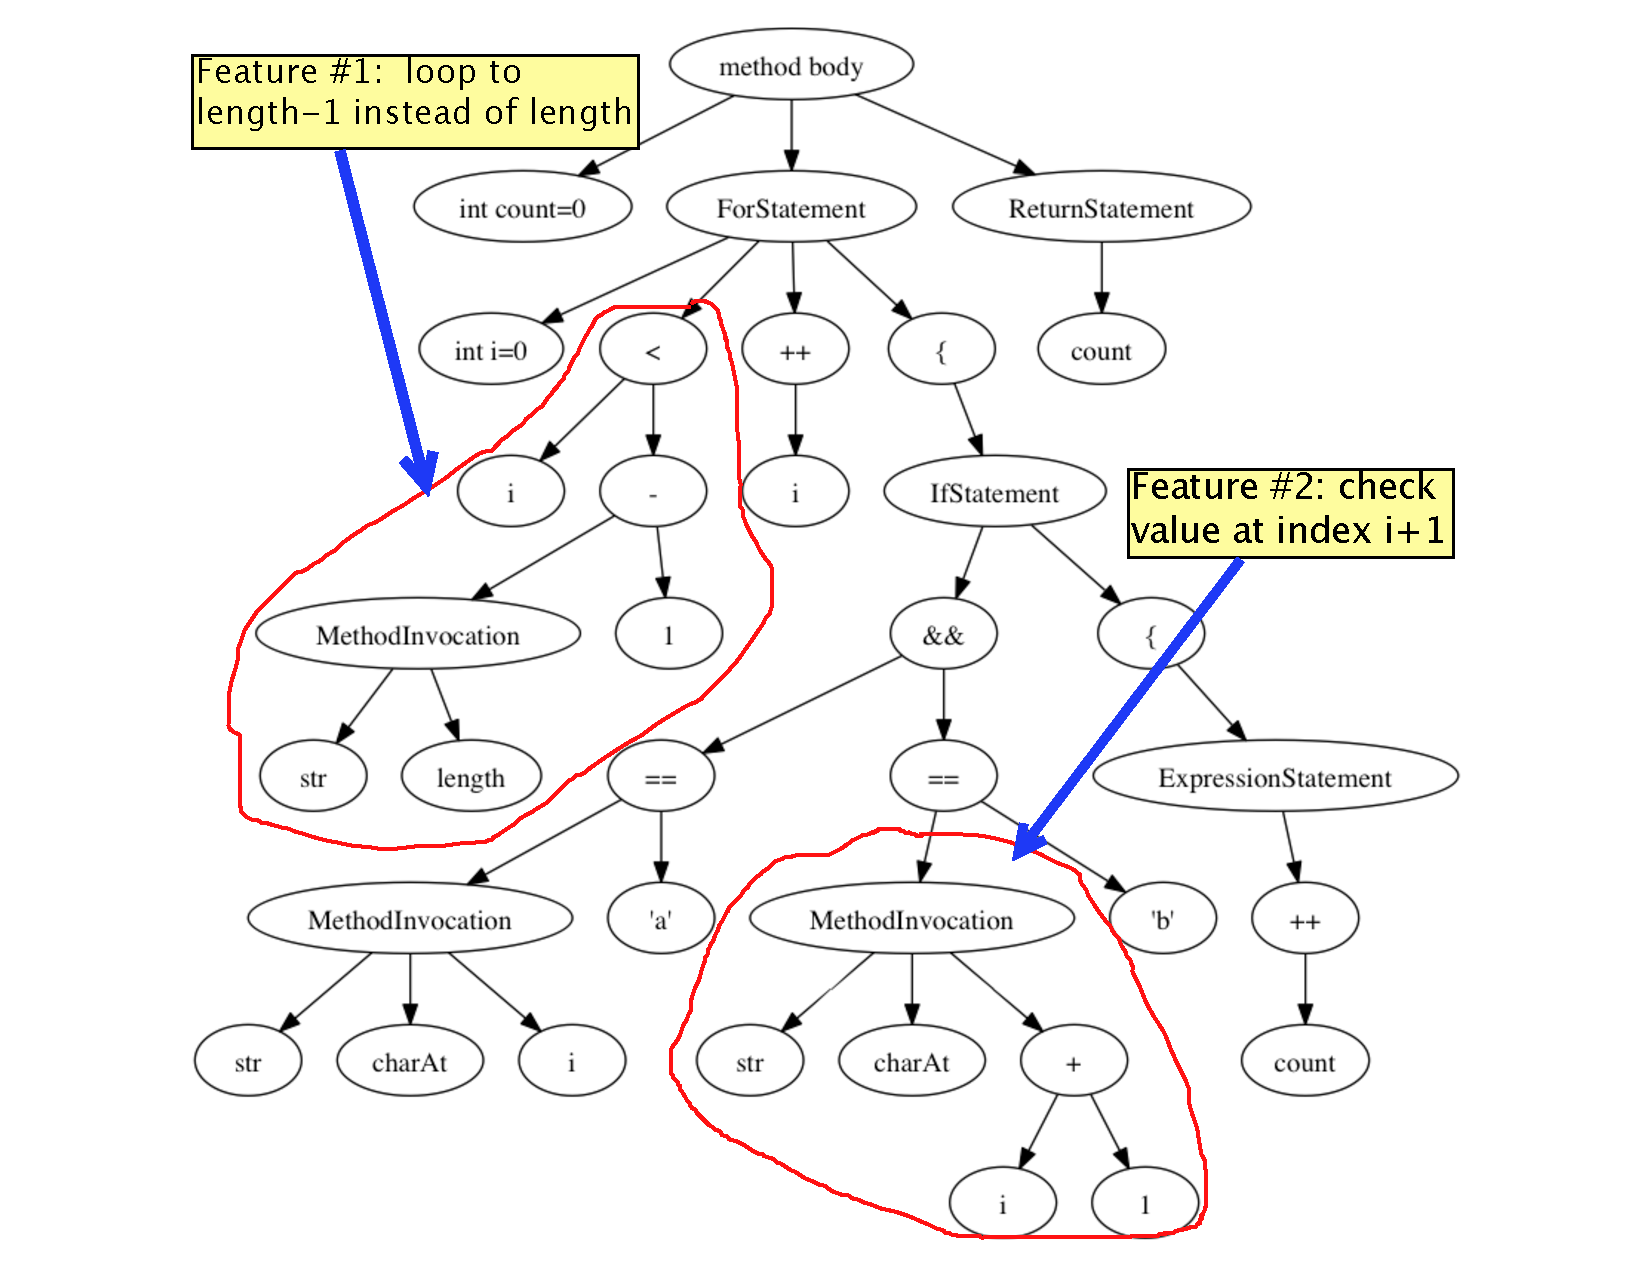
\includegraphics[width=90mm]{images/forloop-highlight}
%\caption{Slightly simplified AST of the code in Figure~\ref{fig:countab-solution}}
%\label{fig:countab-ast}
%\end{figure}
%
%Note the two circled sub-trees, or {\em features}, in the AST depicted
%in Figure~\ref{fig:countab-ast}.  Feature \#1, the {\em
%  length-1} feature, shows the loop iterating
%until the length of the String minus one.  The for loop requires a
%stop condition that is different
%than the loop stop condition used to solve the {\tt CountA} exercise from
%Figure~\ref{fig:counta}.  Crucially, once we know students are
%using a for loop to solve this exercise (which we can also
%extract from the AST), {\em we know exactly where in the AST to
%  look for the length-1 feature}.  If a submission has all the
%features except the {\em length-1} feature, we have a pretty good idea
%that the student hasn't figured out to change the stop condition of the
%for loop.  We could use the lack of features present in correct
%solutions to give us an idea of what things the student is missing.
%
%
%\subsection{Limits of Key Features Approach}
%
%Our approach of identifying ``key features'' has a number of
%weaknesses and limitations.  First, like other ITS hint-systems, it
%requires a reliable system for identifying the nearest previous successful
%submission to a student's current program state.  Work in this area is
%ongoing \cite{rivers-its2012,Jin:2012:PRA:2345840.2345889}.
%
%Second, features are based purely on the structure of the
%code, and are treated independently of one another, which is a
%simplification that throws out a lot of relevant contextual information.  For
%example, a student submission may have two for loops, one of which has
%an if statement nested inside it; our approach cannot determine which
%loop has the if statement inside it.  
%
%Third, we do not perform any data-flow analysis (at least not yet), so
%we cannot identify if particular values are stored in variables.
%
%Next, we require compilable code, which can be a problem for the many
%students who struggle to get their code to compile
%\cite{Denny:2012:SEE:2325296.2325318}.
%
%Finally, while we focused mainly on exercises that required for loops
%to solve, we also assigned a number of exercises that
%use if statements and no loops.  For these exercises, we can figure
%out when students don't have 
%enough structure, such as when they don't have nested if statements
%for an exercise where most people who solves the exercise used nested if statements.  However,
%we cannot yet easily determine when students have the wrong boundary
%conditions in an if statement.
%
%Much more work is needed in this area.  We hope that 
%CloudCoder can help out by providing a rich data set for post-hoc
%studies, as well as a platform for testing out a hint-system.


\bibliographystyle{abbrv}
\bibliography{paper}  

%\appendix
%Appendix A
\section{Acknowledgements}

We would like to thank the anonymous reviewers for helpful suggestions
for improving the paper.

This work was supported by a SIGCSE Special Projects grant (May 2012).

\end{document}
